\documentclass[Royal,times,sageh]{sagej}

\usepackage{moreverb,url,natbib, multirow, tabularx}
\usepackage[colorlinks,bookmarksopen,bookmarksnumbered,citecolor=red,urlcolor=red]{hyperref}



% tightlist command for lists without linebreak
\providecommand{\tightlist}{%
  \setlength{\itemsep}{0pt}\setlength{\parskip}{0pt}}





\begin{document}


\setcitestyle{aysep={,}}

\title{Network Regression on Cosponsorship and Religion in United States
Congress}

\runninghead{Dionne \emph{et al}.}

\author{Natalie Dionne\affilnum{1}, Naomi Liftman\affilnum{2}}

\affiliation{\affilnum{1}{Department of Government, Smith
College}\\\affilnum{2}{Department of Statistical and Data Science, Smith
College}}

\corrauth{Naomi Liftman}

\email{\href{mailto:nliftman@smith.edu}{\nolinkurl{nliftman@smith.edu}}}

\begin{abstract}
Lorem ipsum dolor sit amet, consectetur adipiscing elit. Aenean ut elit
odio. Donec fermentum tellus neque, vitae fringilla orci pretium vitae.
Fusce maximus finibus facilisis. Donec ut ullamcorper turpis. Donec ut
porta ipsum. Nullam cursus mauris a sapien ornare pulvinar. Aenean
malesuada molestie erat quis mattis. Praesent scelerisque posuere
faucibus. Praesent nunc nulla, ullamcorper ut ullamcorper sed, molestie
ut est. Donec consequat libero nisi, non semper velit vulputate et.
Quisque eleifend tincidunt ligula, bibendum finibus massa cursus eget.
Curabitur aliquet vehicula quam non pulvinar. Aliquam facilisis tortor
nec purus finibus, sit amet elementum eros sodales. Ut porta porttitor
vestibulum. Integer molestie, leo ut maximus aliquam, velit dui iaculis
nibh, eget hendrerit purus risus sit amet dolor. Sed sed tincidunt ex.
Curabitur imperdiet egestas tellus in iaculis. Maecenas ante neque,
pretium vel nisl at, lobortis lacinia neque. In gravida elit vel
volutpat imperdiet. Sed ut nulla arcu. Proin blandit interdum ex sit
amet laoreet. Phasellus efficitur, sem hendrerit mattis dapibus, nunc
tellus ornare nisi, nec eleifend enim nibh ac ipsum. Aenean tincidunt
nisl sit amet facilisis faucibus. Donec odio erat, bibendum eu imperdiet
sed, gravida luctus turpis.
\end{abstract}

\keywords{Cosponsorship, Networks, Religion, Polarization}

\maketitle

\hypertarget{introduction}{%
\section{Introduction}\label{introduction}}

Extensive literature supports the importance of cosponsorship as the
core activity in building the legislative agenda. As Schiller (1995)
outlines, sponsorship is one of the few legislative activities which
legislators have almost total control. Legislatures can decide to
introduce and support legislation that appeases their constituents,
progresses their political career, and initiates institutional change on
a variety of policies. While legislators can be thought of as individual
sponsoring and cosponsoring bills, when combined the collaborative
process of agenda setting reflects shared interests and communal values.
The agenda setting stage is believed to be critical in the legislative
process due to its ability to control or manage what issues gain
government attention.

As cosponsorship is the most used tie in the legislative network, there
is a growing body of literature that explores a variety of identity
based characteristics on cosponsorship networks. This research has
focused primarily on political identities (i.e.~partisanship and
political ideology) {[}should i cite who?{]} and visible identity
characteristics (i.e.~age, race, gender, and ethnicity). Both have
provided extensive support of Huckfeldt's (1984) claim that one's
community and one's individual characteristics influence their political
actions.

However, existing scholarship falls short on researching the effects of
religious affiliation on the congressional cosponsorship network. Given
its intrinsic function as a core component of an individual's identity
and its known effect on political ideology (Mctague \& Pearson-Merowitz
2013), there is a theoretical framework that religion influences
legislators actions. This paper provides empirical evidence on how the
congressional cosponsorship network is affected by legislators'
religious identity.

In this paper, we examine the United States 112th Congress (2011-2013)
and the 117th Congress (2021-2023). Data on sponsorship and
cosponsorship (roughly 30,000 bills each session) is used in conjunction
with network analysis to model the influence of religion in each
respective session. We then cross compare the resulting networks to
understand how the effect of religious affiliation on congressional ties
has changed over the past ten years. With this, we also contribute to
the existing body of literature on recent trends in polarization,
specifically the growing political division created by religion.

Figure \ref{fig:plot}

\hypertarget{literature-review}{%
\section{Literature Review}\label{literature-review}}

Figures are supported from R code:

\ldots and can be referenced (Figure \ref{fig:plot}) by including the
\texttt{\textbackslash{}\textbackslash{}label\{\}} tag in the
\texttt{fig.cap} attribute of the R chunk:
\texttt{fig.cap\ =\ "Fancy\ Caption\textbackslash{}\textbackslash{}label\{fig:plot\}"}.
It is a quirky hack at the moment, see
\href{https://github.com/yihui/knitr/issues/323}{here}.

Analogously, use Rmarkdown to produce tables as usual:

\begin{verbatim}
if (!require("xtable")) install.packages("xtable")
\end{verbatim}

\begin{verbatim}
## Loading required package: xtable
\end{verbatim}

\begin{verbatim}
xt <- xtable(head(cars), caption = "A table", label = "tab:table")
print(xt, comment = FALSE)
\end{verbatim}

\begin{table}[ht]
\centering
\begin{tabular}{rrr}
  \hline
 & speed & dist \\ 
  \hline
1 & 4.00 & 2.00 \\ 
  2 & 4.00 & 10.00 \\ 
  3 & 7.00 & 4.00 \\ 
  4 & 7.00 & 22.00 \\ 
  5 & 8.00 & 16.00 \\ 
  6 & 9.00 & 10.00 \\ 
   \hline
\end{tabular}
\caption{A table} 
\label{tab:table}
\end{table}

Referenced via \ref{tab:table}. You can also use the YAML option
\texttt{header-includes} to includes custom \LaTeX packages for tables
(keep in mind that \texttt{pandoc} uses \texttt{longtables} by default,
and it is hardcoded; some things may require including the package
\texttt{longtable}). E.g., using \texttt{ctable}:

\begin{verbatim}
header-includes:
- \usepackage{ctable}
\end{verbatim}

Then, just write straight-up \LaTeX code and reference is as usual
(\texttt{\textbackslash{}ref\{tab:ctable\}}):

\begin{verbatim}
\ctable[cap = {Short caption},
        caption = {A caption for this table.},
        label={tab:ctable},]
        {cc}
        {
        \tnote[$\ast$]{Footnote 1}
        \tnote[$\dagger$]{Other footnote}
        \tnote[b]{Mistakes are possible.}
        }{
        \FL
        COL 1\tmark[a] & COL 2\tmark[$\ast$]
        \ML
        6.92\tmark[$\dagger$] & 0.09781 \\
        6.93\tmark[$\dagger$] & 0.09901 \\
        97 & 2000
        \LL
}
\end{verbatim}

It is also possible to set the \texttt{YAML} option
\texttt{longtable:\ true} and use markdown tables (or the
\texttt{knitr::kable} function): \texttt{knitr::kable(head(cars))}
produces the same table as the \texttt{xtable} example presented before.

\hypertarget{cross-referencing}{%
\subsection{Cross-referencing}\label{cross-referencing}}

The use of the Rmarkdown equivalent of the \LaTeX cross-reference system
for figures, tables, equations, etc., is encouraged (using
\texttt{{[}@\textless{}name\textgreater{}{]}}, equivalent of
\texttt{\textbackslash{}ref\{\textless{}name\textgreater{}\}} and
\texttt{\textbackslash{}label\{\textless{}name\textgreater{}\}}). That
works well for citations in Rmarkdown, not so well for figures and
tables. In that case, it is possible to revert to standard
\LaTeX syntax.

\hypertarget{double-spacing}{%
\subsection{Double Spacing}\label{double-spacing}}

If you need to double space your document for submission please use the
\texttt{doublespace} option in the header.

\hypertarget{bibliography}{%
\section{Bibliography}\label{bibliography}}

Link a \texttt{.bib} document via the YAML header, and bibliography will
be printed at the very end (as usual). The default bibliography style is
provided by Wiley as in \texttt{WileyNJD-AMA.bst}, do not delete that
file.

Use the Rmarkdown equivalent of the \LaTeX citation system using
\texttt{{[}@\textless{}name\textgreater{}{]}}. Example:
\citep{Taylor1937}, \citep{Knupp1999, Kamm2000}.

To include all citation from the \texttt{.bib} file, add
\texttt{\textbackslash{}nocite\{*\}} before the end of the document.

\hypertarget{further-information}{%
\section{Further information}\label{further-information}}

All \LaTeX enviroments supported by the main template are supported here
as well; see the \texttt{.tex} sample file
\href{http://onlinelibrary.wiley.com/journal/10.1002/(ISSN)1097-0258/homepage/la_tex_class_file.htm}{here}
for more details and example.

\begin{verbatim}
print(x)
\end{verbatim}

\begin{figure}
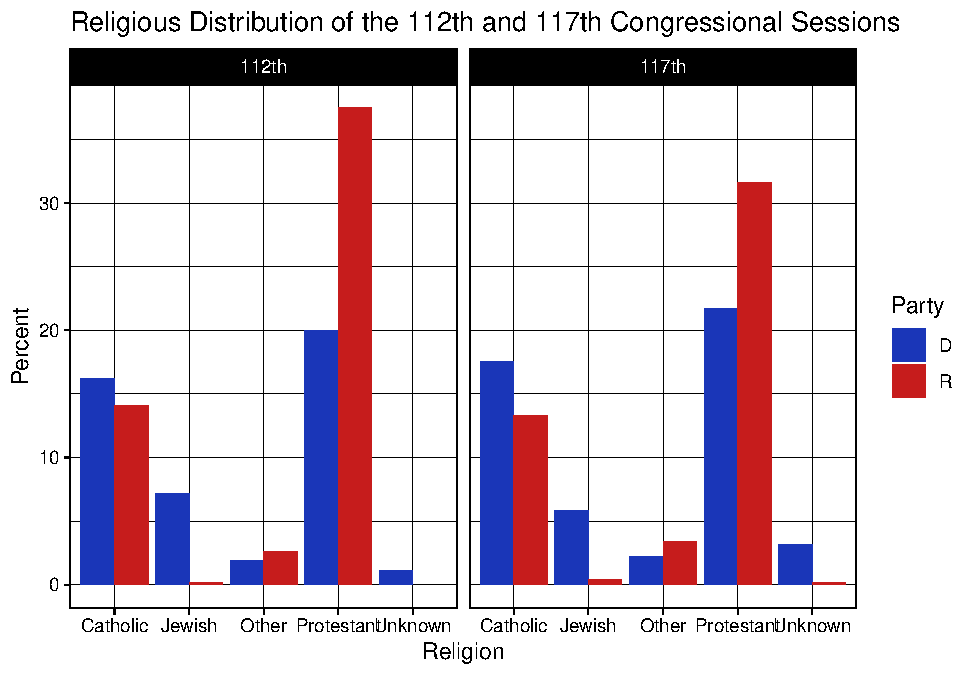
\includegraphics[width=1\linewidth]{Final-Report_files/figure-latex/plot-ref-1} \caption{Fancy Caption\label{fig:plot}}\label{fig:plot-ref}
\end{figure}

\bibliographystyle{sageh}
\bibliography{bibfile}


\end{document}
